% !TeX root = ../thuthesis-example.tex

\chapter{\MakeUppercase{The VR-IoT Research Platform}}

In this chapter, we introduce key implementation details and the architecture of the VR-IoT research platform, or, as it was later named, ``NUIX-Studio.''

\section{Platform requirements}

Based on the first meeting discussion \cite{tsinghua_hci_lab_nuix-studio_2021}, it was decided that the main functions of the platform would include:
\begin{enumerate}
     \item Visualization of devices;
     \item Interaction with devices;
     \item Simulation of device sensors.
\end{enumerate}

Our platform must provide an interface for different interaction techniques and simulation of device sensors inside Virtual reality. The device controls can be divided between touch interface interaction and other interaction methods, such as voice control, sight control, gesture control, etc. The ability to control devices at a distance impossible in real life, such as lengthening arms, dropping hands, etc., was placed in a separate category. These control methods could be used in the real world in the future by introducing new technologies such as holographic projection.

Based on the literature review, the platform should fulfill these minimum requirements:
\begin{enumerate}
\item Scalability. The performance of the platform should stay acceptable when the number of devices in the system increases. Otherwise, the latency of the synchronization between the devices inside the VR-IoT environment will increase to a level at which the system is unable to perform Data analysis for the research;
\item Ease of use and testing. Researchers need to be able to efficiently use the NUIX-Studio API and platform tools to create new IoT devices and test them in the VR-IoT environment.
\item Fault Tolerance. The platform should effectively handle faults coming from both real and virtual worlds to provide a satisfying user experience;
\item Simultaneous work. As in the real world, where several people can interact with an IoT system at the same time, each of the platform's running instances should be able to operate simultaneously and with the same data.
\end{enumerate}

By dividing the NUIX-Studio structure into these three layers, the platform becomes more resilient (Figure~\ref{fig:BasicPlatformStructure-figure}): 
\begin{enumerate}
    \item Real-world IoT devices HUB is a special device responsible for receiving and sending data to real-world devices that provides the data in a unified format (through the abstraction of sensors) for the middle layer. An open-source software openHAB~\cite{OpenHab} is used to support different IoT devices. The HUB runs on a server and is responsible for storing the IoT devices' data. The data is managed through a Web Interface;
    \item Integration layer is responsible for analyzing data coming from VR and the real-world, integrating real-world device data into VR (and vice-versa), performing persistence, and providing an API for using the platform in research projects. By receiving and sending unified data objects representing the IoT devices' sensor data using REST API calls, each of the NUIX-Studio App instances operates with the same data, enabling simultaneous work. The next step is to represent the IoT devices' data in Virtual reality and perform computations for research. Since the platform should run smoothly on VR headsets and provide good UX, the analysis should be performed on a powerful PC\footnote{In Chapter 4 an experiment proving this statement is provided.}. At the same time, Virtual reality headsets perform computations for interacting with objects, such as hand recognition;
    \item Visualization layer. Interaction with digital IoT devices can be performed using VR headsets, AR devices, or by simulating touch, sight, gestures, and other interactions. The platform provides an API for developers to integrate their interaction techniques into this layer, but developing these techniques is not the focus of this research. We decided to use Unity~\cite{Unity} for interaction with virtual reality devices. Firstly, Unity comes with a ready-to-use 3D engine, relieving the need to develop a new one. Secondly, Unity is multi-platform and supports VR headsets. Thirdly, developers are already familiar with Unity development, making it easier for them to integrate the platform into their solutions.
\end{enumerate}

\begin{figure}
  \centering
  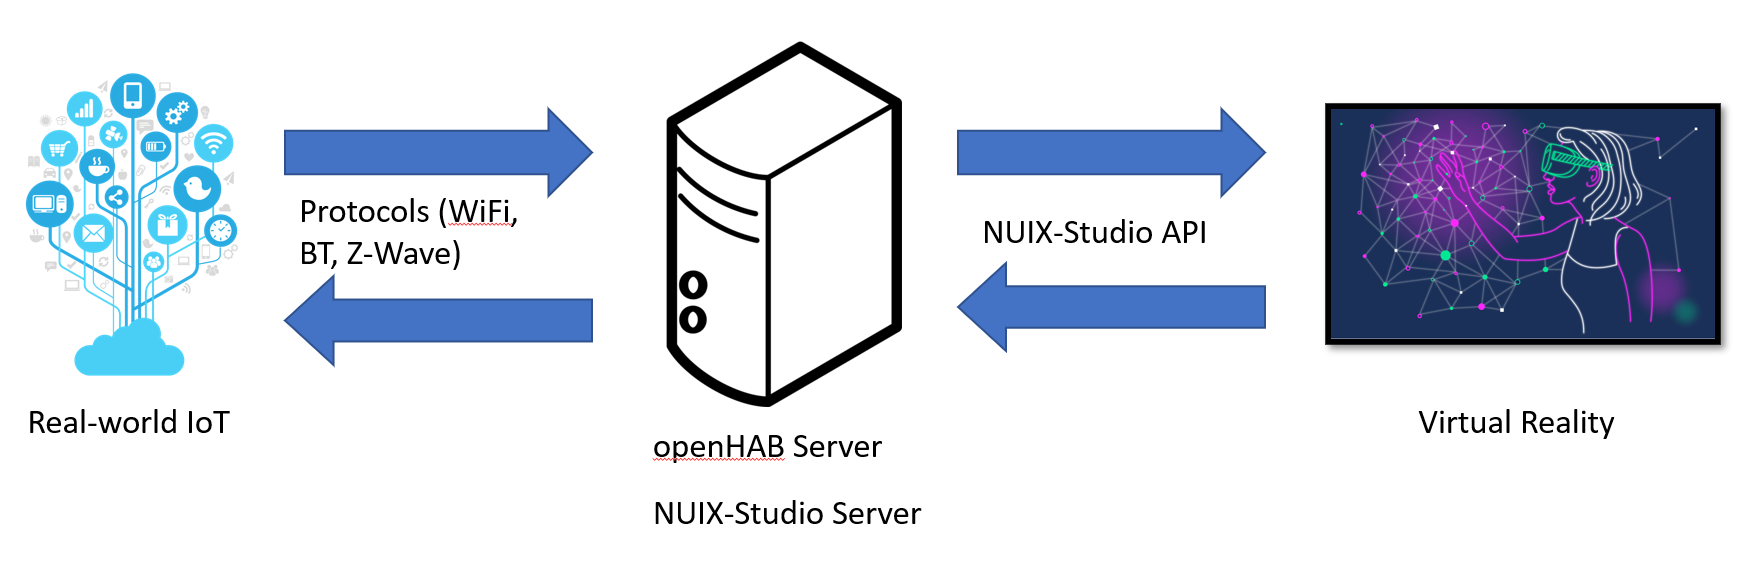
\includegraphics[width=0.9\linewidth]{figures/BasicPlatformStructure.png}
  \caption{Simplified structure of NUIX Studio. The real-world IoT devices HUB is an openHAB server, while NUIX-Studio server is an instance of the NUIX-Studio App responsible for the computations.}
  \label{fig:BasicPlatformStructure-figure}
\end{figure}

\subsection{Platform structure}

As it can be seen on the IoT-VR Platform design architecture, the Real-world IoT devices Hub should collect the data coming from IoT Services and store it in a database (Figure~\ref{fig:StructureVersion2-figure}). It should be able to synchronize the data with the integration layer, complementary linking real and virtual sensing data.

\begin{figure}
  \centering
  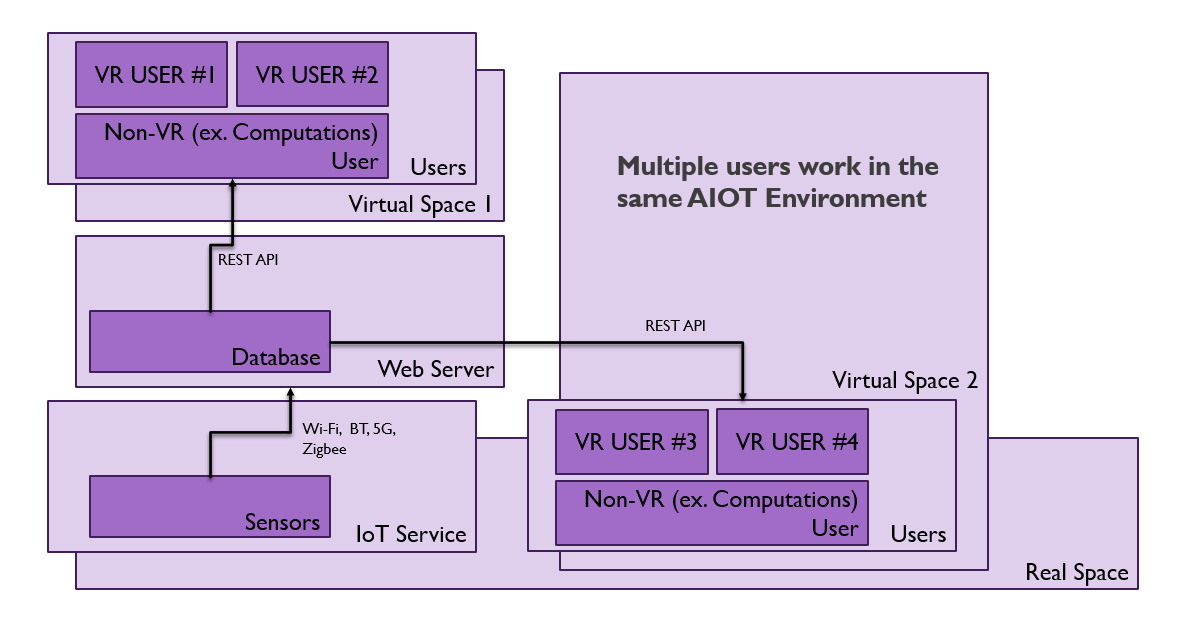
\includegraphics[width=0.9\linewidth]{figures/StructureVersion2.png}
  \caption{Design architecture of the platform for virtuality-reality synchronization and simultaneous work support.}
  \label{fig:StructureVersion2-figure}
\end{figure}

\section{Server architecture}

\subsection{OpenHAB Server Structure}

We decided not to change the openHAB system's structure, because it already follows the SOA principles that allow implementing support for various types of devices (Figure~\ref{fig:openHABServerStructure-figure}).

\begin{figure}
  \centering
  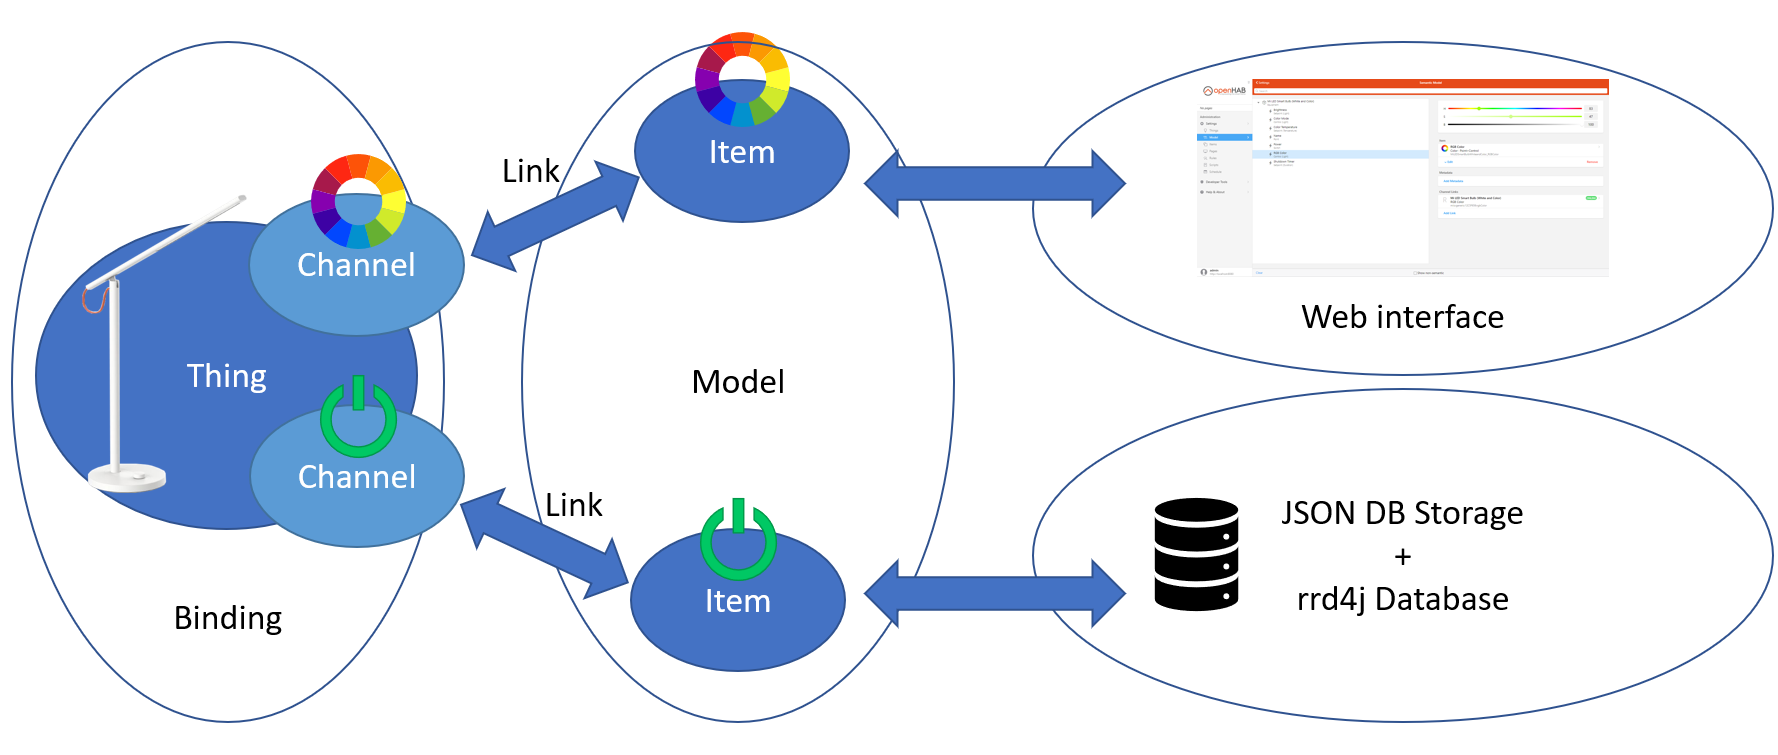
\includegraphics[width=0.9\linewidth]{figures/openHABServerStructure.png}
  \caption{Server structure}
  \label{fig:openHABServerStructure-figure}
\end{figure}

Each IoT device is called a Thing, but a Thing can also be a service. For example, a smoke sensor or a user location are both Things.

Things expose their capabilities through Channels. For example, smart vacuum cleaner channels can be suction strength, water delivery strength, remaining charge level, and cleaning status.

Each channel is associated with one or more Items that are added inside the model. In the example, each of the Items is linked to only one Channel, and each of the channels is linked to only one Item. Items have a State, and they may receive commands. 

Before adding an IoT device to the server, the developer has to first install a software adapter. These add-ons are called Bindings, and they provide a way to link Items to physical devices. Most of the protocols for connecting to IoT devices are supported by the corresponding Bindings.

For example, after a Binding for Xiaomi smart home devices is installed, the smart home devices can be automatically discovered by the server and added as Things. A Xiaomi Lamp is used in the example, for which several Channels are presented (Figure~\ref{fig:XiaomiLampChannels-figure}).

\begin{figure}
  \centering
  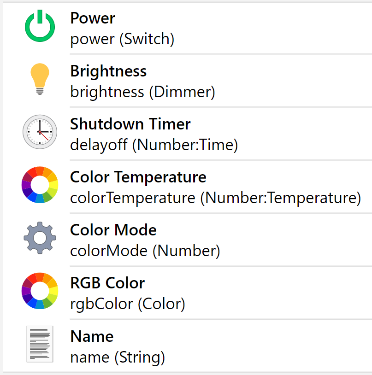
\includegraphics[width=0.6\linewidth]{figures/XiaomiLampChannels.png}
  \caption{Channels list example.}
  \label{fig:XiaomiLampChannels-figure}
\end{figure}

Each of these channels represents one Item (Figure~\ref{fig:XiaomiLampPowerItem-figure}).

\begin{figure}
  \centering
  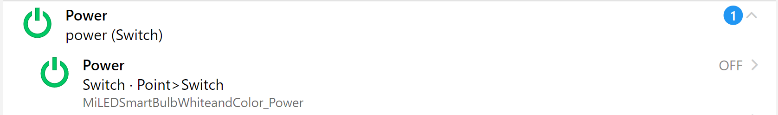
\includegraphics[width=0.9\linewidth]{figures/XiaomiLampPowerItem.png}
  \caption{An Item example.}
  \label{fig:XiaomiLampPowerItem-figure}
\end{figure}

For example, the Power Control is performed through the power channel. In terms of the introduced concepts, the Power Control is an Item named ``MiLEDSmartBulbWhiteandColorPower'' of type Switch and State ``OFF.''

As soon as the lamp is turned On, the Power Control switch in the Web Interface will also turn ON. And if the switch is changed to the ``OFF'' state in the Web Interface, the lamp will automatically turn off.

\subsection{Server Extended Structure}

In the previous section, it was not specified how the platform should access the server data. Syncing is performed through REST API (Figure~\ref{fig:ExtendedServerStructure-figure}) , which is explained in detail in Table~\ref{tab:rest-api-table}.

\begin{figure}
  \centering
  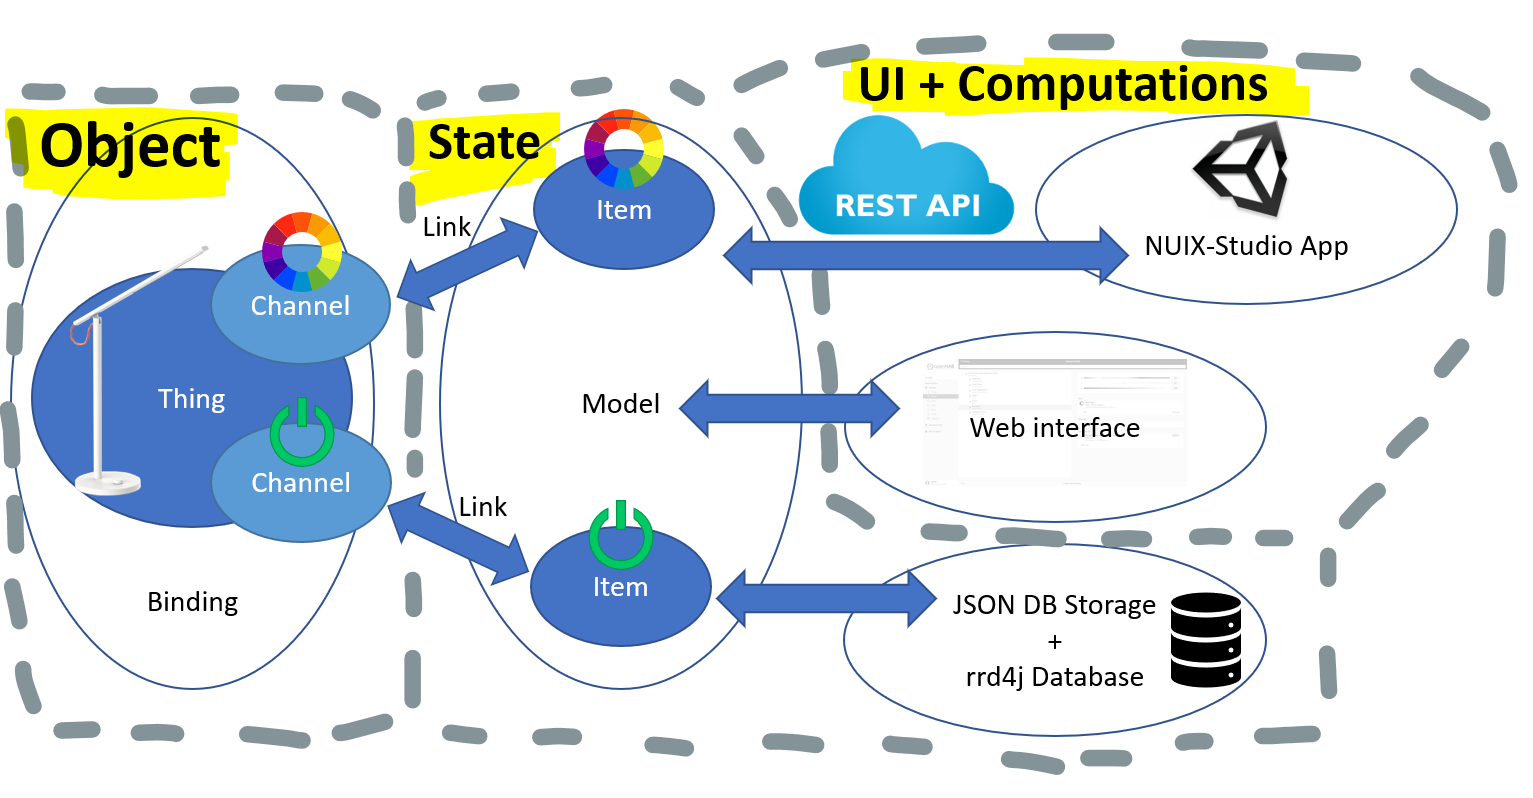
\includegraphics[width=0.9\linewidth]{figures/ExtendedServerStructure.png}
  \caption{Structure of the server showing how the NUIX-Studio App connects to it.}
  \label{fig:ExtendedServerStructure-figure}
\end{figure}

\begin{table}
  \centering
  \begin{threeparttable}[c]
    \caption{REST API commands used in NUIX-Studio}
    \label{tab:rest-api-table}
    \begin{tabular}{ll}
      \toprule
      REST API CALL    &         DESCRIPTION                 \\
      \midrule
      GET\tnote{a} & Get all available items \\
      POST\tnote{b} & Adds a new item to the registry or updates the existing item    \\
      PUT\tnote{b}        & Sends a command to the item                              \\
      DELETE\tnote{b}        & Removes an item from the registry          \\
      \bottomrule
    \end{tabular}
    \begin{tablenotes}
      \item [a] For link: /items
      \item [b] For link: /items/<itemname>
    \end{tablenotes}
  \end{threeparttable}
\end{table}

In the current implementation of the platform, four different REST API commands are used: GET command for receiving Items in the registry on system startup, PUT command to create a new Item on the server, POST command for updating the state of the Item, and DELETE command for removing an Item from the server.

States of the Items are received by getting events from the server: once the event is received, the Item state can be retrieved from the Data Transfer Object's (DTO) payload.

\section{The platform architecture}

As mentioned above, there can be several NUIX-Studio App instances running at the same time. Each of them has access to the Server through REST API. The instances can be of one of the three types:

\begin{enumerate}
    \item Virtual Reality Instance. It runs on Oculus or another VR headset and has remote or local access to the server. Items received from the server are visualized. It is possible to interact with the Items in different ways by touching buttons, moving sliders, performing hand gestures, using voice commands, etc. 
    \item Computations Instance. It runs on a powerful machine and has either remote or local access to the server. Since latency is important for the VR-IoT platform's performance, it is preferable to run this instance on the same machine as the openHAB server. In this case, the REST API calls time will be less than the minimum measurement unit (compared to milliseconds for accessing remote virtual reality instances)\footnote{An experiment to prove this statement is provided in Chapter 4.}. Physics, Big Data analysis, and other performance-based computations are executed in this instance, while user interactions are limited.
    \item Input simulation instance. If the App instance runs on the device with limited support of virtual reality interaction interfaces (for example, a PC), input simulation can be used. Sometimes, it is even easier to run and test the platform on such devices: for example if using a physical keyboard is required or if there is no access to a VR headset.
\end{enumerate}

Each of the instances has access to the same data on the server, making it possible to work simultaneously in one virtual environment and divide tasks between several NUIX-Studio App instances (Figure~\ref{fig:AppInstances-figure}). One of the instances can be used for computations, while others can be used for interacting with the devices in Virtual reality.

\begin{figure}
  \centering
  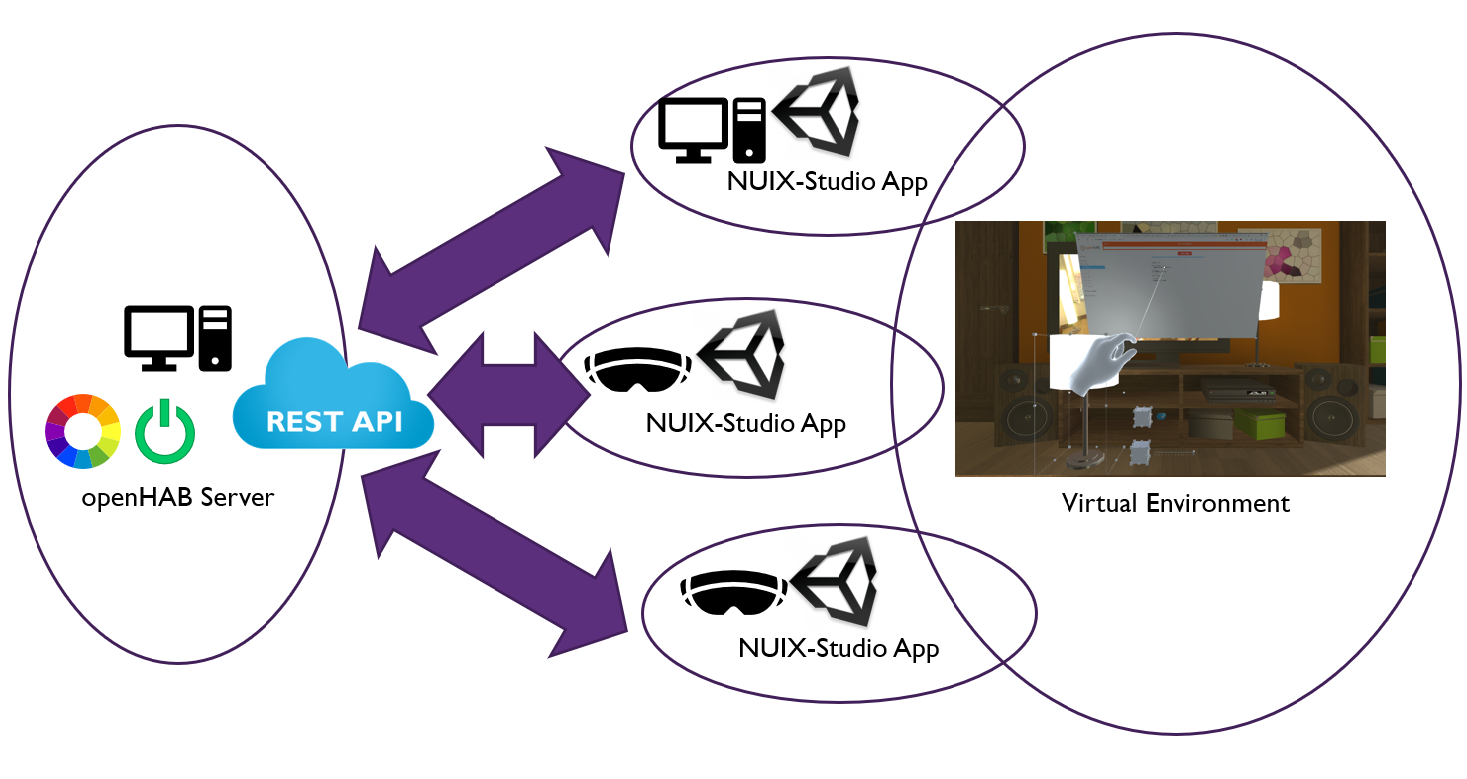
\includegraphics[width=0.9\linewidth]{figures/AppInstances.png}
  \caption{NUIX-Studio App Instances}
  \label{fig:AppInstances-figure}
\end{figure}

\subsection{NUIX-Studio App Architecture}

After the NUIX-Studio App requests access to the system to get the list of items from the registry, a list of Item Data Transfer Objects is received by the App and then added into the Semantic Model (Figure~\ref{fig:AppArchitecture-figure}). After the Item state is updated or an Item is added or removed, an event is sent to the EventController instance, and then, based on the event payload, the Item list is updated.  By keeping the Item data on the device equal to the Item data on the server, the Semantic model in the NUIX-Studio App remains equivalent to the Semantic model presented on the server. 

\begin{figure}
  \centering
  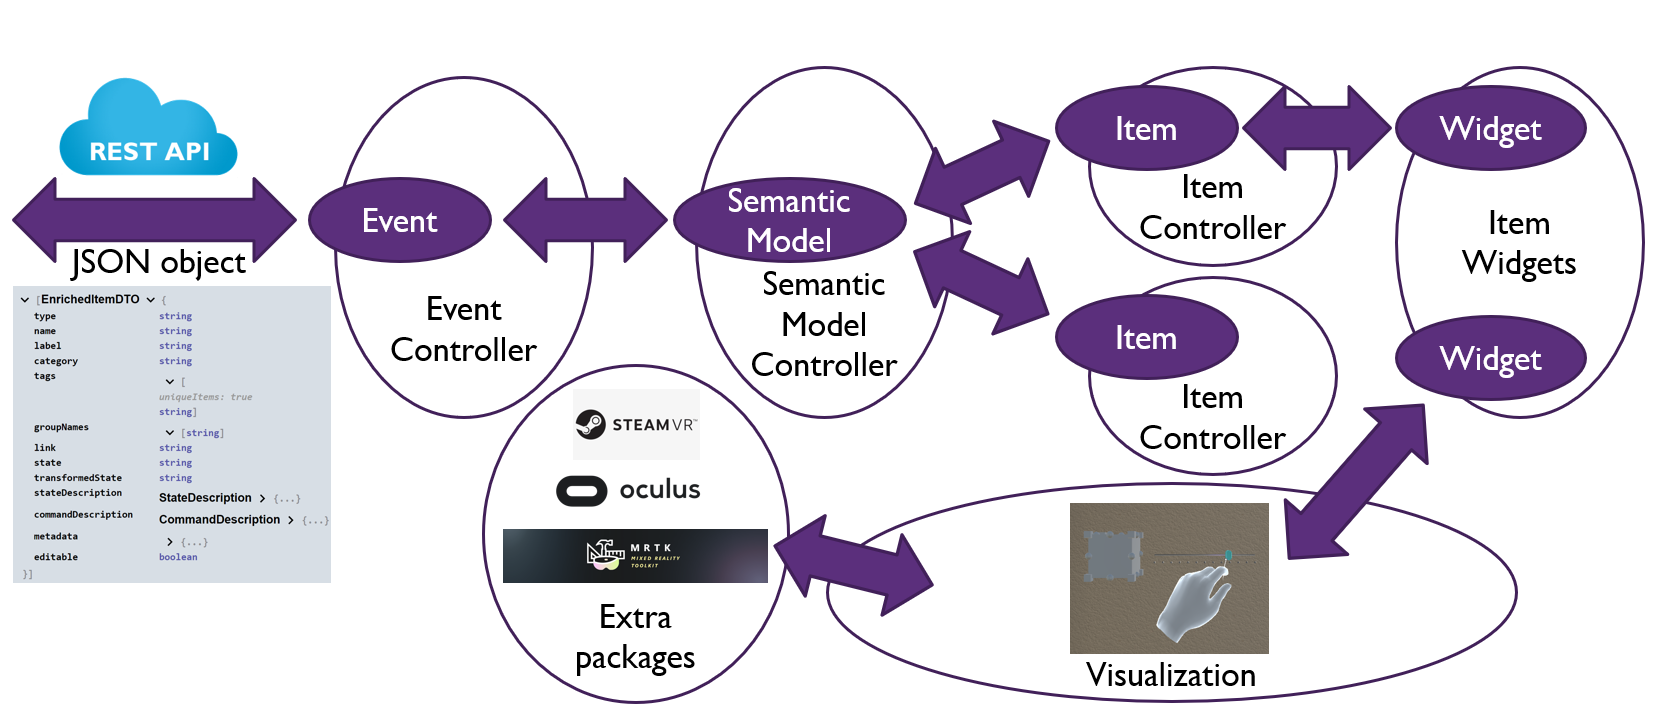
\includegraphics[width=0.9\linewidth]{figures/AppArchitecture.png}
  \caption{NUIX-Studio App Architecture}
  \label{fig:AppArchitecture-figure}
\end{figure}

But if the states of the Items are only stored in the App, users will not be allowed to interact with the IoT devices. In other words, the NUIX-Studio App has to provide an interface to interact with the Items. Since different types of Items require different interaction techniques, a Widget object is created for each item type.
Widget in NUIX-Studio App is a Unity Virtual object, which can visualize the Item state and update it. For example, it can be an interactable pinch slider for a dimmer Item or a virtual screen for an Image item.

By integrating Extra frameworks, the NUIX-Studio platform can provide a wider variety of Widgets and a higher number of supported devices. For example, Oculus Integration support provides an API for hand recognition; SteamVR~\cite{SteamVR2021} support makes it possible to run the NUIX-Studio App on the majority of VR headsets.

\subsection{NUIX-Studio App Semantic Model}

As mentioned above, the Semantic model in the NUIX-Studio App is kept equivalent to the Semantic model stored on the server. The advantages of this approach are listed below:

\begin{enumerate}
    \item Each of the App instances visualizes equivalent data, providing simultaneous and fault-tolerant work;
    \item The Semantic model on the server is time- and memory-effective. Hence, the Semantic model in the App is also time- and memory-effective.
\end{enumerate}

Overall, using the defined approach, the platform doesn't depend on concretions, and both the Semantic model and Item are abstractions.

But when it is necessary to provide an interface for creating new IoT devices in VR and to interact with them, the Items presented on the server only cannot be used. For example, each Item's virtual position inside the VR environment is a piece of required data that should be accessible by each of the instances.

The platform's main purpose is to provide an interface to test new IoT devices inside Virtual reality or extend the existing items with extra functionality. But only real-world devices' data is stored on the server. Therefore, the Semantic model should be extended with extra items.

\section{Devices representation}

Compared to the existing solutions on the market, this is the first solution to automatically add any device from the real world to Virtual reality.

A functional solution for IoT research requires support for various types of devices. Although the IoT market has numerous different devices, the general device parameters values can be specified. Following the definitions given in this chapter, each device is represented as a Thing and includes several Items. Thus, each device existing or created in the future can be divided into blocks in terms of the VR-IoT Research Platform architecture. The supported Item types are listed in the Table~\ref{tab:items-table}.

\begin{table}
  \centering
  \begin{threeparttable}[c]
    \caption{The supported Item types}
    \label{tab:items-table}
    \begin{tabular}{ll}
      \toprule
      ITEM TYPE    &         DESCRIPTION                 \\
      \midrule
      Color &	RGB Color value \\
      Contact & Whether the sensors are located close enough to each other \\
      DateTime & Date and time parameters \\
      Dimmer &	Dimmer value in percentage \\
      Group &	An Item containing other Items \\
      Image &	The binary data of an image \\
      Location & GPS Coordinates \\
      Number & Value stored in number format \\
      Number:<dimension> & Number Item with specified unit support \\
      Player & Item that control video, audio playback \\
      String &	Text or binary data \\
      Switch & Boolean value \\
      \bottomrule
    \end{tabular}
  \end{threeparttable}
\end{table}

The universal Item is String since the data collected by IoT sensors can be represented in binary format in almost all cases. Hence, the data operated on by IoT devices can be placed inside Item blocks.

After the NUIX-Studio App receives the Item of a specific format, the Semantic model is updated. Next, the Item's corresponding Widgets are updated as well.


\section{Platform prototyping}

As written in the beginning of this chapter, the platform should fulfill the minimum requirements of scalability, ease of use and testing, fault tolerance and simultaneous work support. Following these conditions was one of the platform development main tasks. Each next prototype was closer than the previous one to following the requirements. In total, five prototypes have been developed. Further, key features of each of the prototypes are given.

\subsection{Platform distribution}

The platform's source code is hosted at NUIX-Studio~\cite{NUIXStudio} repository. The source code distribution required keeping the repository size at a minimum while providing an easy installation procedure. NUIX-Studio was shared as a separate package to meet these requirements.

\subsection{Platform prototype 1 and 2}

The first and second NUIX-Studio prototypes did not initially support Virtual reality (Figure~\ref{fig:Prototype2-figure}).

\begin{figure}
  \centering
  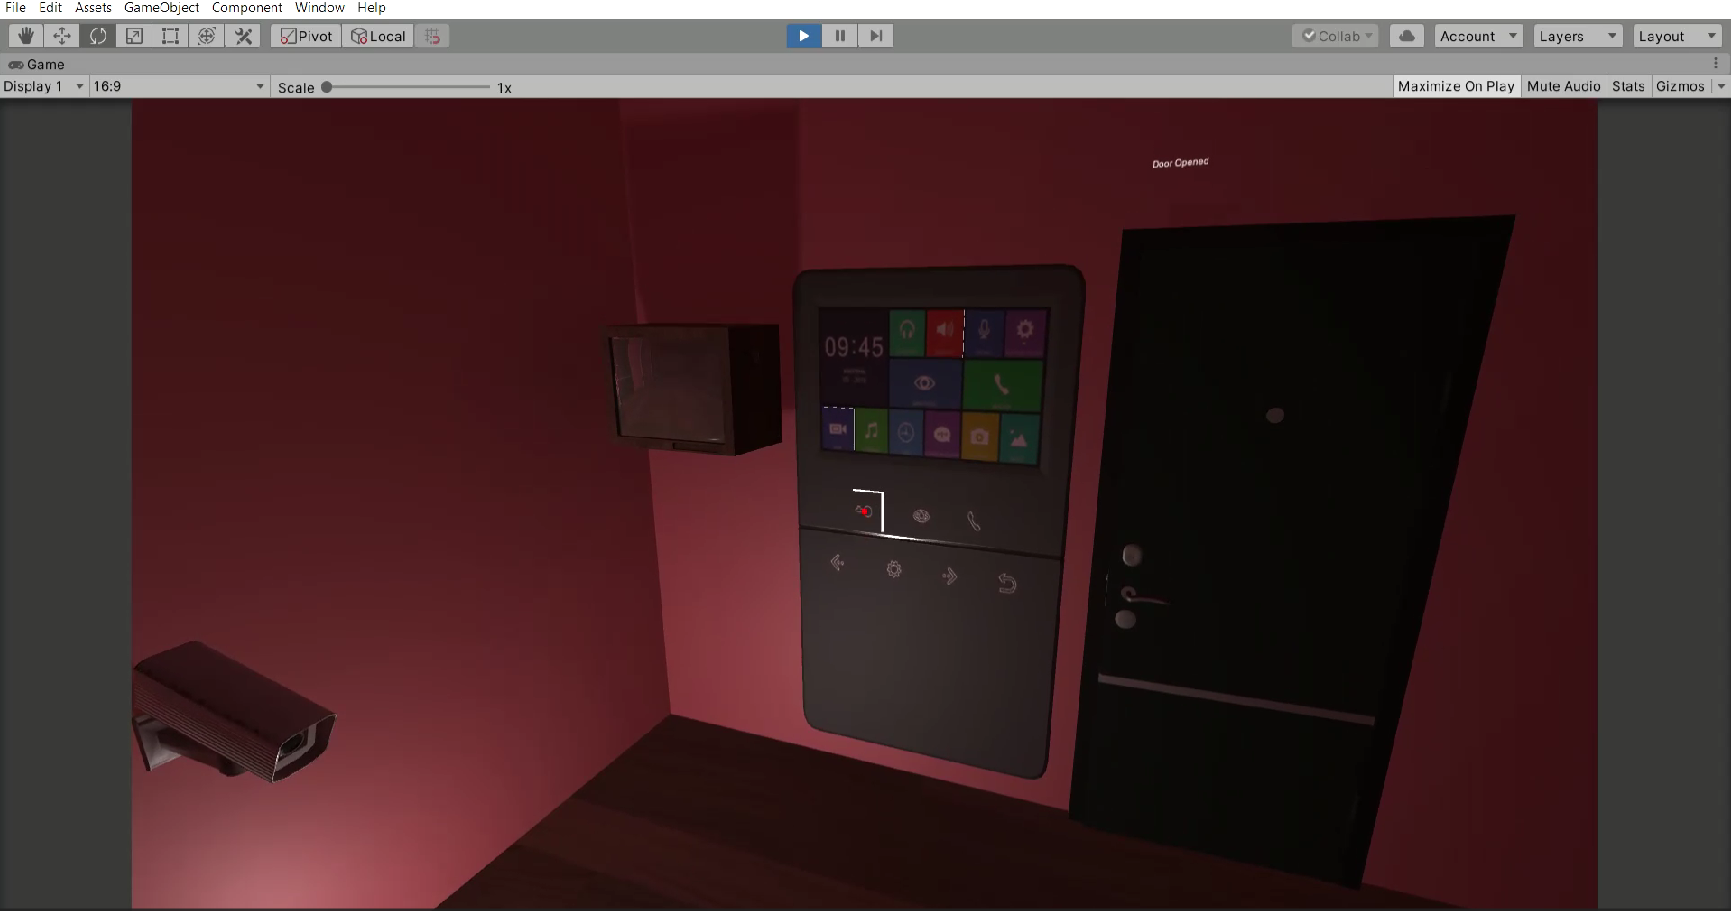
\includegraphics[width=0.9\linewidth]{figures/Prototype2.png}
  \caption{The second prototype of the VR-IoT Research platform}
  \label{fig:Prototype2-figure}
\end{figure}

The only possible interface to interact with the virtual IoT devices was computer mouse. Hence, only basic ways to operate the IoT devices were provided, such as Sight sensing or pressing the buttons. However, the Widgets for device sensing and visualization were implemented (Door open/close sensor, virtual Camera, virtual Speaker).

\subsection{Platform prototype 3}

The key feature of this prototype was the support of Oculus Integration package. While keeping the number of external dependencies to minimum, the platform already provided an API for research in AIoT environment.

The final structure used in NUIX-Studio is different from the structure in Figure~\ref{fig:Prototype3Structure-figure}. The server was responsible for storing and synchronizing item parameters and maintaining all the Unity-specific functionality of the previous prototypes. The Unity Integration package's job was to create Item representations for Virtual reality and share them to other NUIX-Studio App instances as Unity objects. This approach's main limitation is that Unity objects have a much bigger size than the Data Transfer Objects (DTO) used in the final prototype. These Unity objects were synchronized for every frame of the simultaneous work, which dramatically reduced the NUIX-Studio App instances' performance and made the solution not scalable.

\begin{figure}
  \centering
  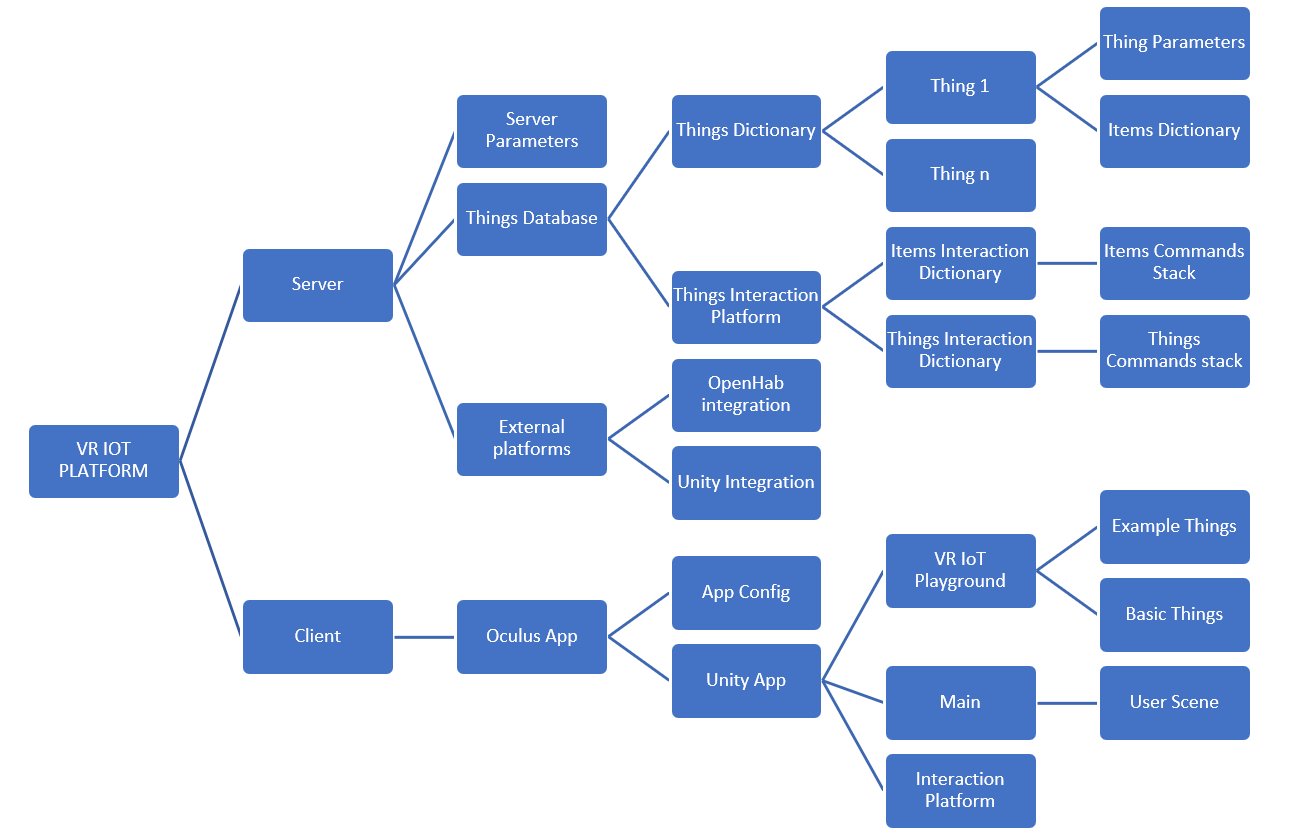
\includegraphics[width=0.9\linewidth]{figures/Prototype3Structure.png}
  \caption{The third prototype's structure}
  \label{fig:Prototype3Structure-figure}
\end{figure}

\subsection{Platform prototype 4}

The third prototype provided only a button Widget (Figure~\ref{fig:Prototype3-figure}), but after integrating Mixed Reality Toolkit into the fourth prototype (Figure~\ref{fig:Prototype4-figure}), additional Widgets were added to the platform. In the fourth prototype, a virtual copy of the real-world Smart home environment was used with virtual items added, such as location, contact, player, switch, and dimmer. Also, several Widgets were supported: sight sensor, motor, light widget, pressure sensor, video streaming screens, and gesture recognition.

\begin{figure}
  \centering
  \subcaptionbox{The third prototype of the VR-IoT Research platform. Button Widget.\label{fig:Prototype3-figure}}
    {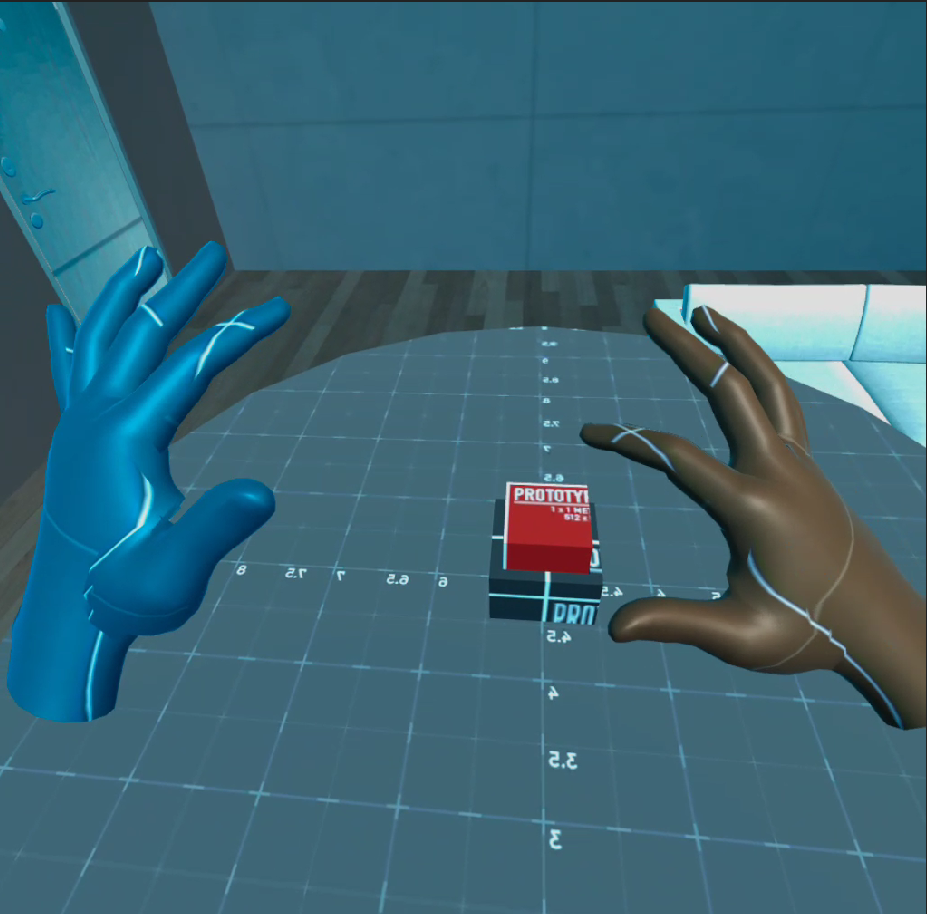
\includegraphics[width=0.435\linewidth]{figures/Prototype3.png}}
  \subcaptionbox{The fourth prototype of the VR-IoT Research platform.\label{fig:Prototype4-figure}}
    {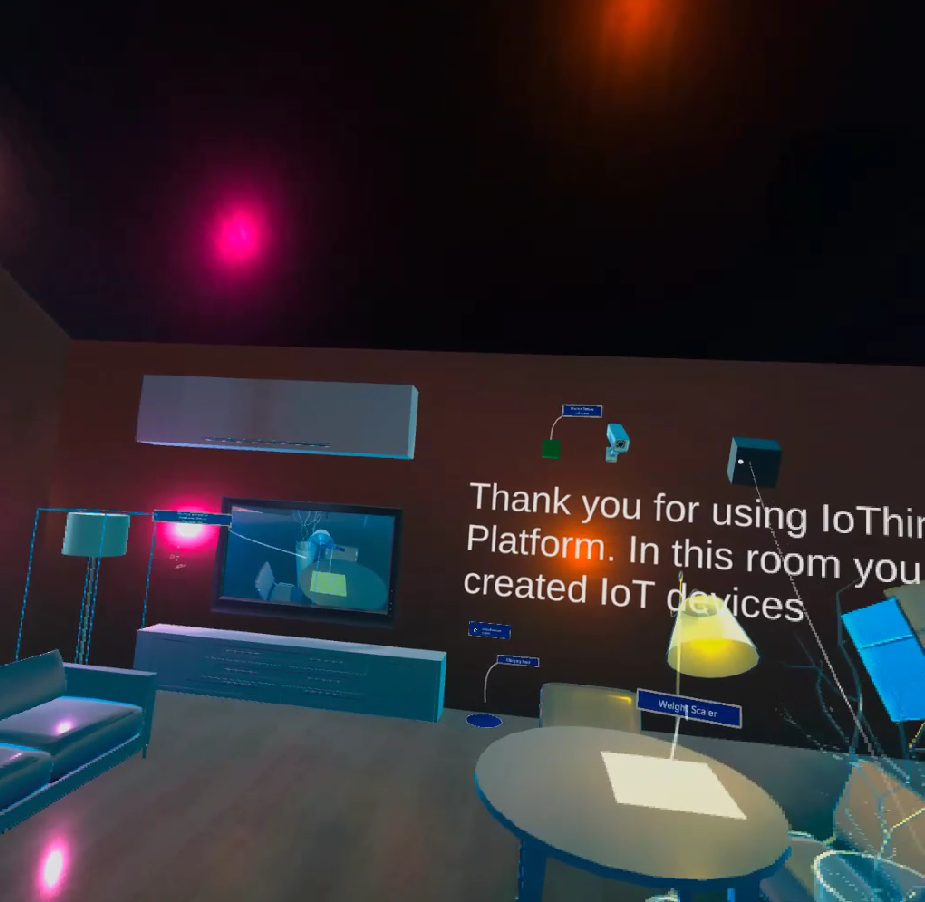
\includegraphics[width=0.44\linewidth]{figures/Prototype4.png}}
  \caption{Prototypes of the UNIX-Studio App.}
  \label{fig:NUIXStudioPrototypes-figure}
\end{figure}

Another important feature added in the fourth prototype was the Input Simulation Service (Figure~\ref{fig:InputSimulation-figure}). In most previous cases, testing the interaction with Widgets required using a Virtual Reality Headset. To use an Oculus Quest VR Headset, developers need to prepare their workplace. Firstly, the environment for using the Virtual Reality Headset must be well lit, otherwise, the Virtual Reality Headset's position detection in the world space will not work correctly. Secondly, the developer must have sufficient amount of space around him to be able to move his Virtual Reality Headset controllers or hands freely. Unfortunately, these requirements for setting up the environment are often infeasible. With the help of the Input Simulation Service system, based on the Mixed Reality Toolkit, it became possible not only to move inside the virtual world but also to make movements with virtual hands, including simulating the various gestures.

\begin{figure}
  \centering
  \subcaptionbox{Pinching gesture simulation\label{fig:InputSimulation-a}}
    {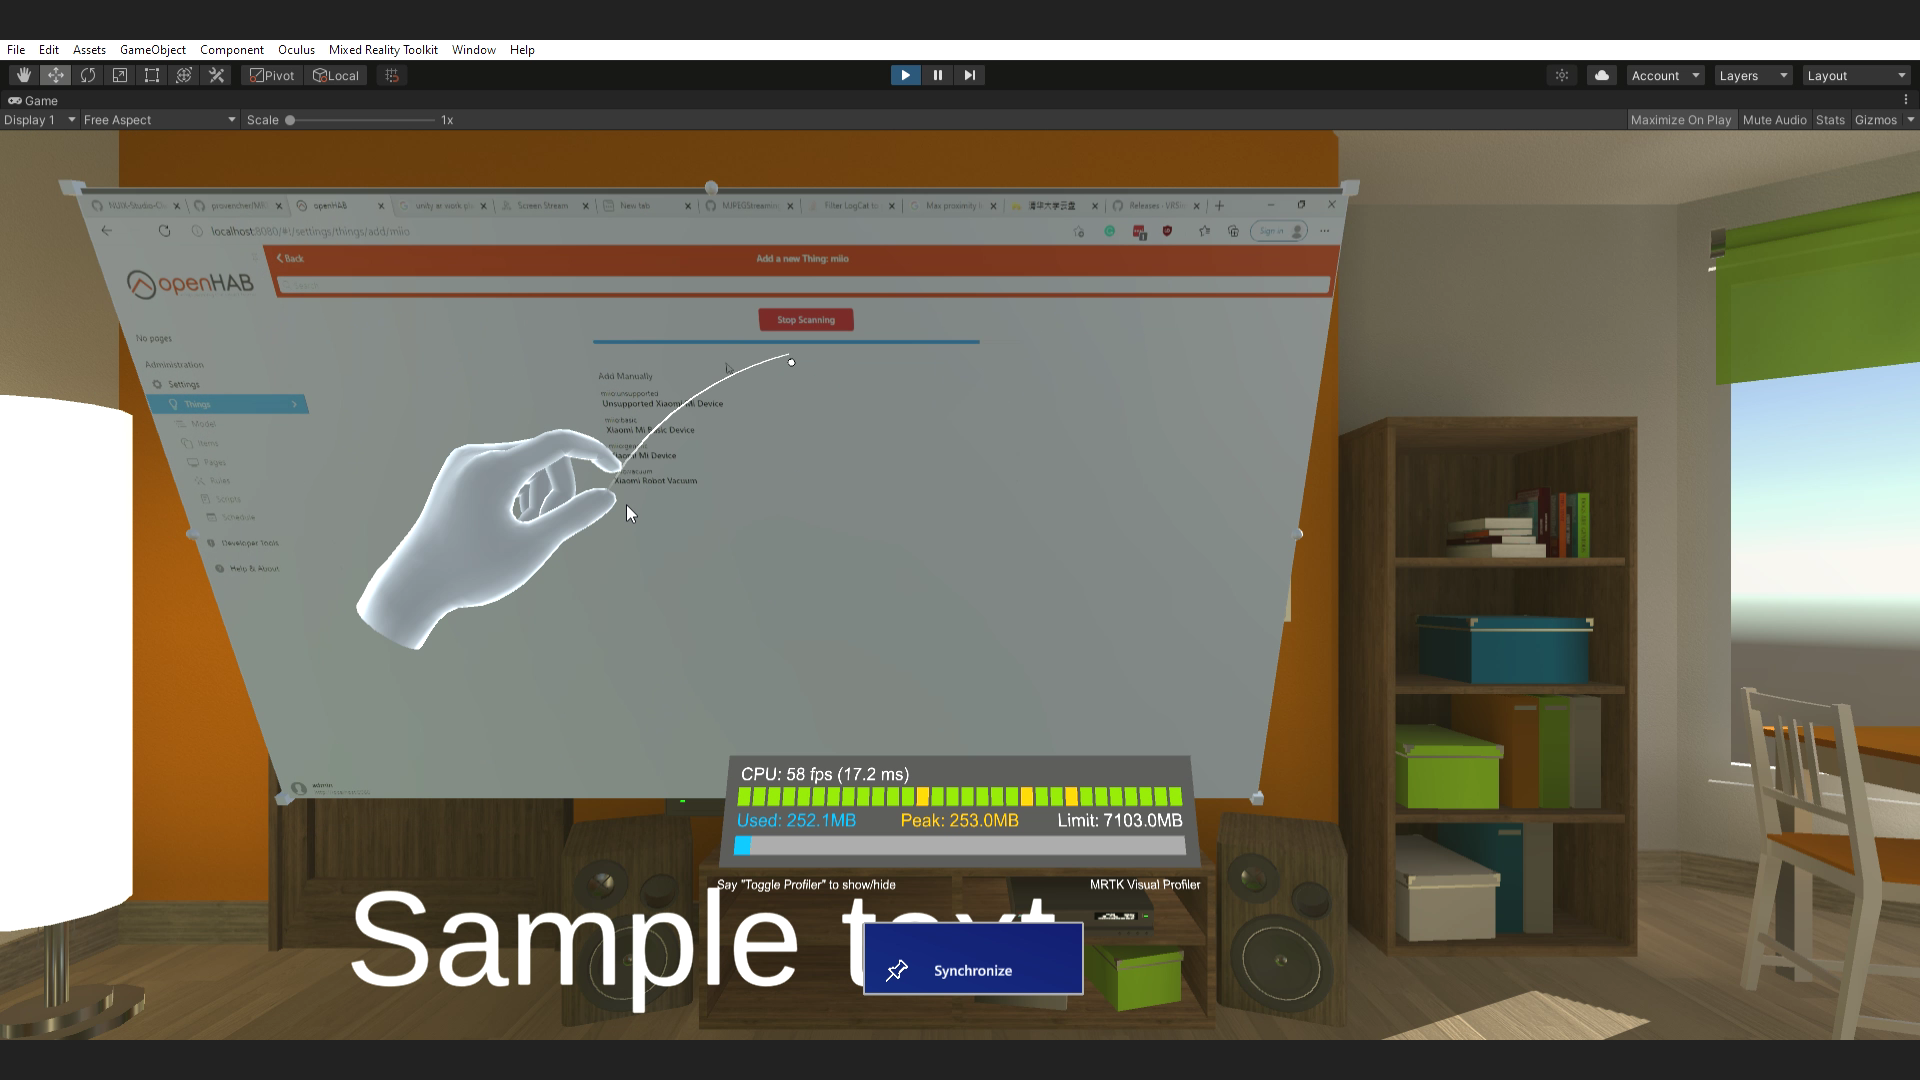
\includegraphics[width=0.45\linewidth]{figures/InputSimulation1.png}}
  \subcaptionbox{Pointing Gesture simulation\label{fig:InputSimulation-b}}
    {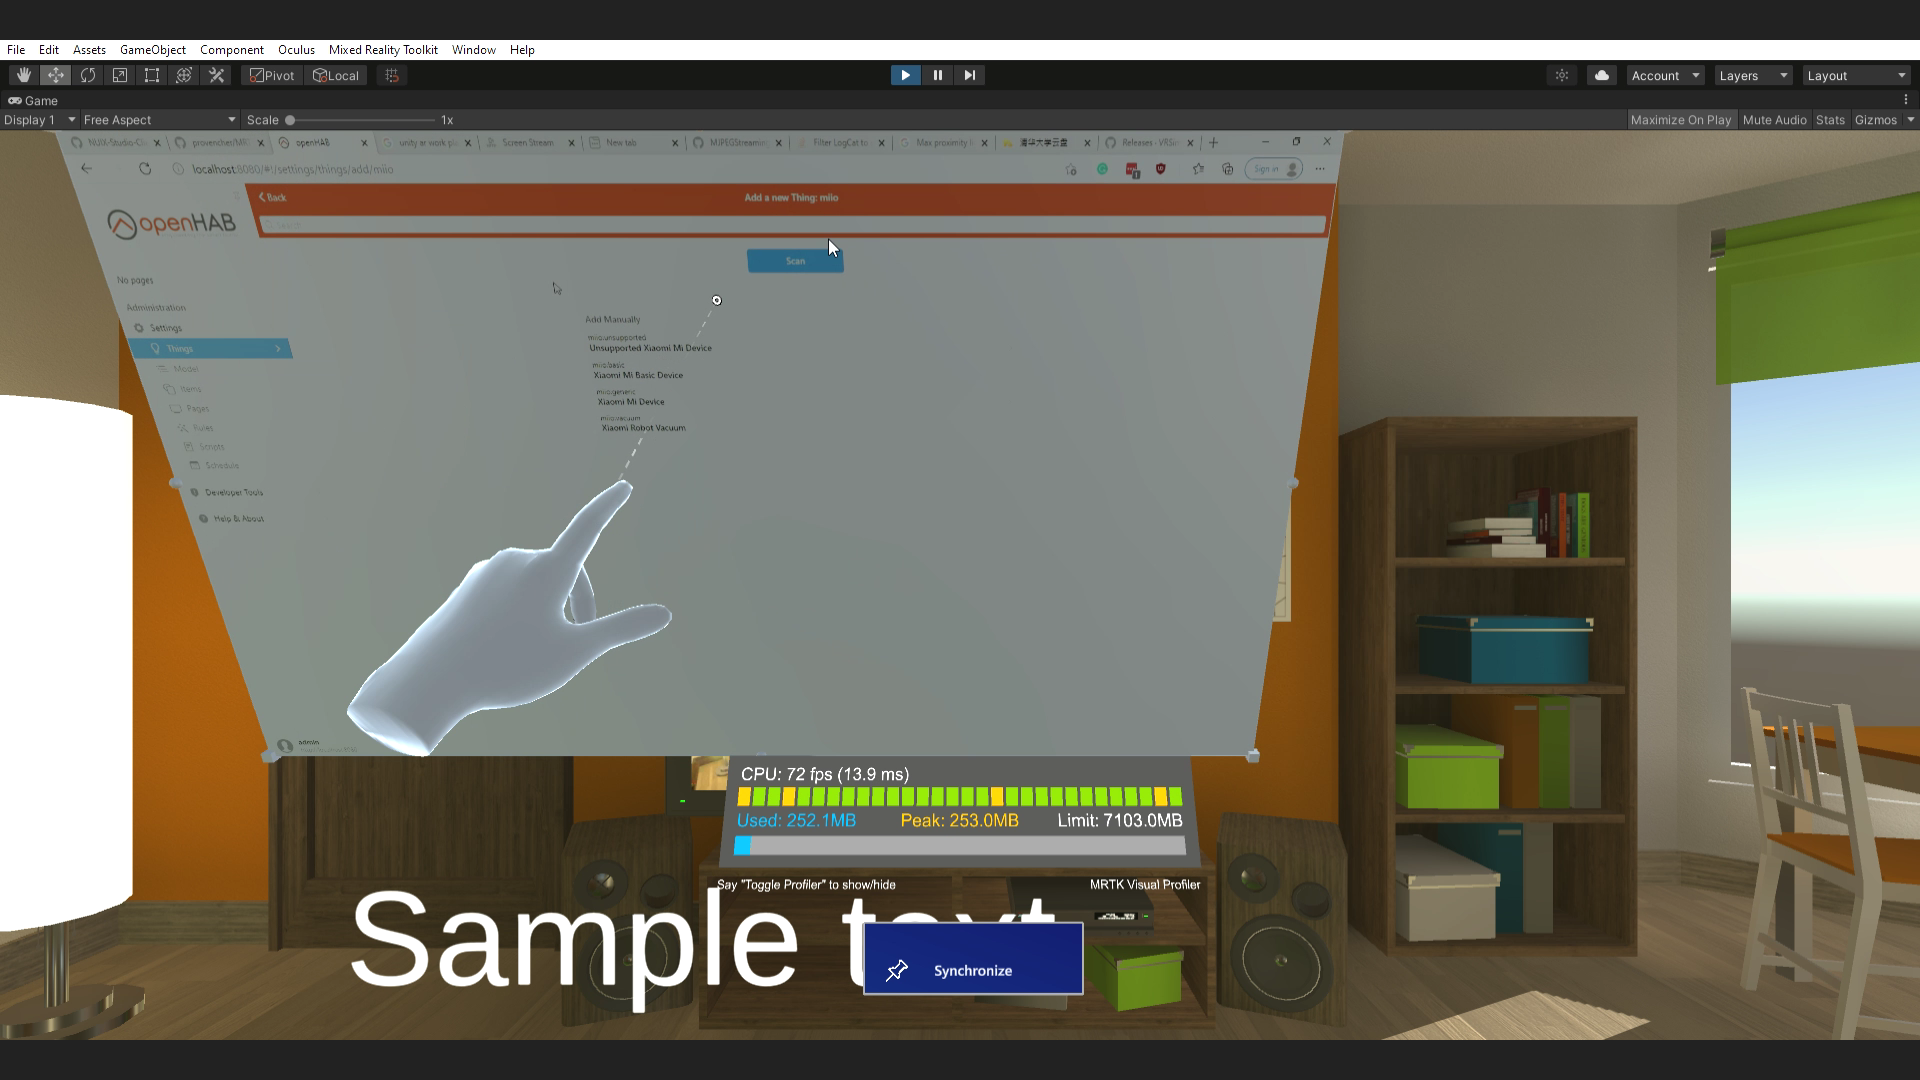
\includegraphics[width=0.45\linewidth]{figures/InputSimulation2.png}}
  \caption{Simulations of gestures on the UNIX-Studio App running on a PC.}
  \label{fig:InputSimulation-figure}
\end{figure}

 Overall, building UX for the IoT devices became easier, but the architecture of the platform remained inefficient. The limitations of this structure kept the platform not scalable and not possible to be used for multiple user scenarios. However, it became easier to use the platform by the people familiar with Unity compared to the Prototype 3.

\subsection{Platform prototype 5}

In the final prototype (Figure~\ref{fig:FinalPrototypes-figure}), the code for most of the items has been rewritten to support the new architecture defined in this chapter. 

\begin{figure}
  \centering
  \subcaptionbox{Typing on the virtual keyboard. \label{fig:FinalPrototype-figure}}
    {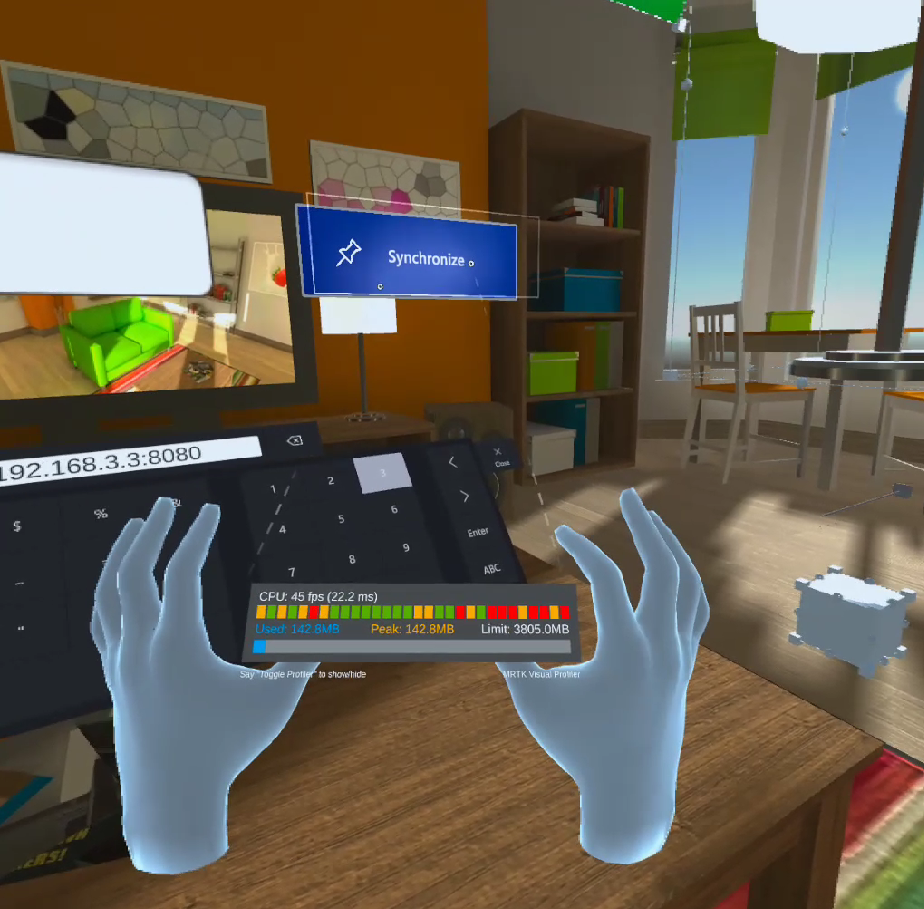
\includegraphics[width=0.45\linewidth]{figures/FinalPrototype.png}}
  \subcaptionbox{Virtual smartphone streaming image from the real smartphone.\label{fig:Prototype5-figure}}
    {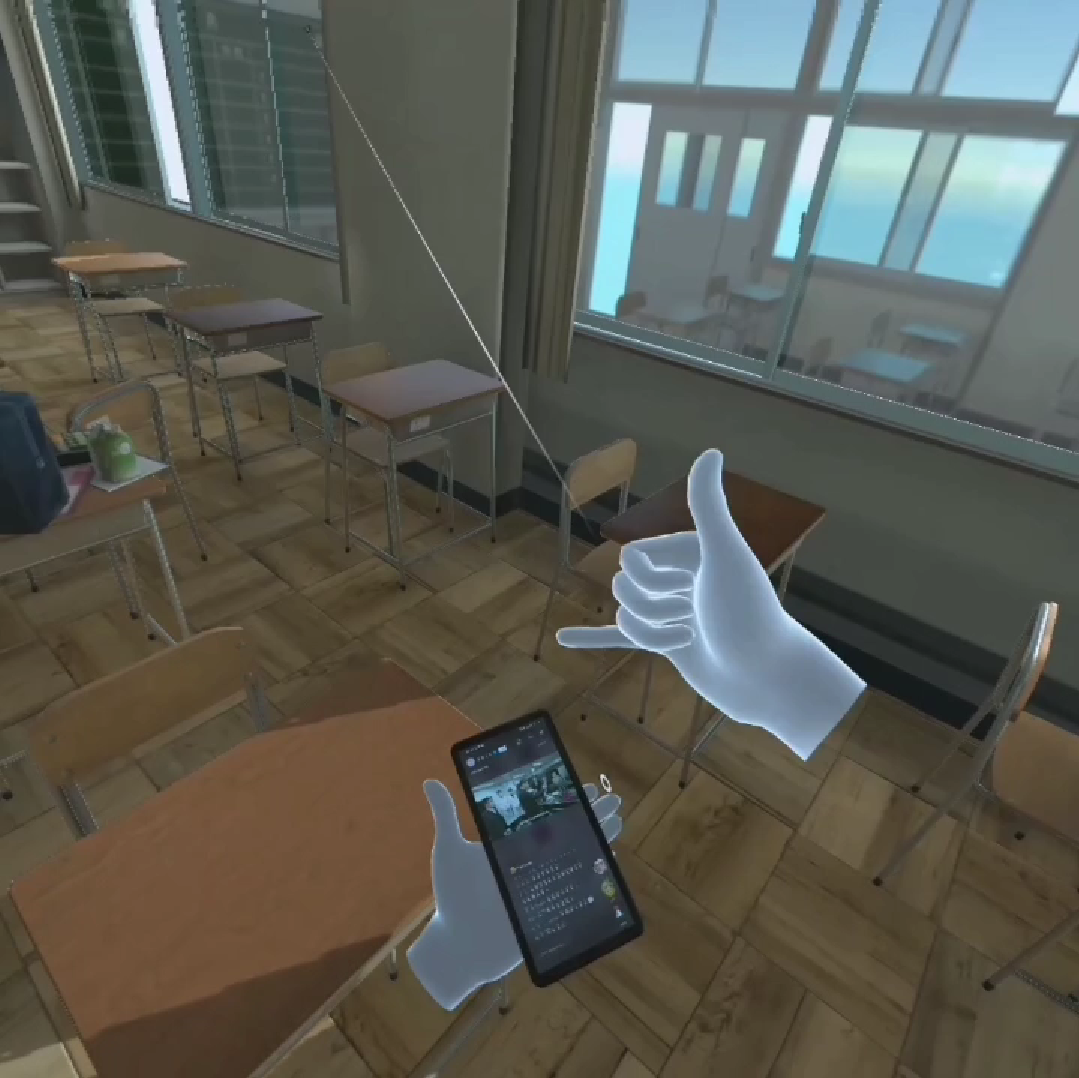
\includegraphics[width=0.45\linewidth]{figures/Prototype5.png}}
  \caption{Screenshots of the final prototypes of the NUIX-Studio App.}
  \label{fig:FinalPrototypes-figure}
\end{figure}

The other changes in the fifth prototype are:
\begin{enumerate}
    \item Performance improvements. By optimizing rendering for Oculus Quest, the framerate in the same scene (Smart home environment) has increased from 30 to over 72 frames per second;
    \item Updated dependencies. Mixed reality toolkit new features support has been added;
    \item Simplified installation. Packages for integration of Oculus and Mixed Reality toolkit have been added to the main project;
    \item Extended documentation. Each Widget's functionality has been summarized. Researchers got better explanation of how to create their own Widgets.
\end{enumerate}

The IoT devices tolerance faults could be successfully handled by openHAB server. The platform itself became easier to use. In the next chapter we introduce NUIX-Studio Development kit, which significantly minimizes the time for research in AIoT scenarios. 